 \subsection{Effect of Device Parameters on Discriminating Capability}
\mynote{HA}{Change heading of figure to say Rhythm ID and PRL+W and not medtronic and BSC}
ICDs have a number of parameters which can be tuned to accommodate specific patient conditions by the physicians. 
%For example, pacemakers have over 400 possible settings for which the physician may tune less than 5 parameters during implantation and in follow-up visits, while leaving the other settings at their default values.
Currently there are very few clinical results on the effect of tuning parameters and their effect on sensitivity and specificity~\cite{maditrit}.
One of the main causes of VT/SVT mis-classifications is inappropriate parameter settings~\cite{wrong_sensing}.
In order for the physicians to set appropriate parameters, it is very important to understand how the change of one parameter can affect the discriminating capability of the device.
It is costly to experiment this on real patients.
With MBCT, one can use the same population across multiple devices with different parameter settings at virtually no cost. 
%The resulting trends can provide valuable insights to physicians.

In this section, we use MBCT to demonstrate the effects of changing two common parameters on SVT/VT discrimination specificity.
The first parameter is the \emph{\textbf{duration}} of arrhythmia before the ICD makes a therapy decision. 
For Boston Scientific ICD the value can be set to 1 to 30 seconds.
In this experiment we explore the values \{1,2,3,4,5,8,10\}.
The equivalent parameter for Medtronic ICD is the number of consecutive fast ventricular intervals which can be set from 8 to 20 beats.
In this experiment we explore the values \{8,10,12,16,18,24,30\} which roughly correspond to the parameters of Boston Scientific ICD.
Intuitively, with a longer duration the device can examine a longer history of the arrhythmia episode, and also allows a greater chance for the arrhythmia to self-terminate. 
This can prevent inappropriate therapy.
Setting the duration too long can also delay and in some cases withhold appropriate therapy. 
These results are in agreement with the recently conducted ADVANCE-III RCT which showed that longer arrhythmia detection windows reduce shocks for Medtronic ICDs~\cite{advance3}.

The second parameter we varied is the \emph{\textbf{VF threshold}}.
For both devices, if the ventricular rate is faster than the VF threshold for a period of time the devices will deliver therapy without going into the SVT/VT discrimination algorithm. So a higher VF threshold means that more signals are passing through the discrimination algorithm.
In this experiment we explored the values \{170,184,200\} for both algorithms.
Intuitively the higher the threshold, the more episodes will be examined by the SVT/VT discrimination algorithm, which may increase specificity.
%However, VTs with rate less than the threshold may also be classified as SVT, causing missed therapies.\\
\newline\textbf{Conducting the Model-based Clinical Trial}. 
For each of the 21 parameter combinations described above, we ran a MBCT with 11,400 EGM episodes on both device models. 
%Each MBCT took approximately 3 hours on a 3GHz Intel Xeon processor with 8 cores. The resulting specificity values are shown in Fig. \ref{fig:parameter}. 
From the results we observe that for both algorithms the specificity increases monotonically with the length of the duration.
When the duration is longer than 5, sensitivities dropped below 100\%, which is in line with the intuition.
\begin{figure}[t]
	
		\centering
		\vspace{-10pt}
		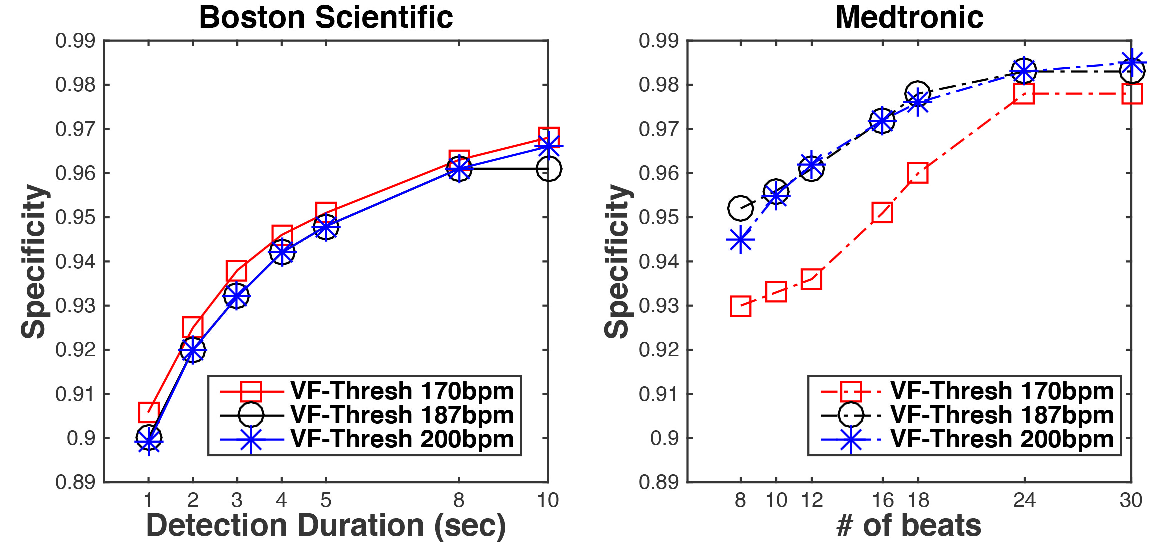
\includegraphics[width=0.45\textwidth]{figs/parameter.pdf}
		\caption{\small Effects of Duration and VF threshold parameters on Specificity}
		\vspace{-10pt}
		\label{fig:parameter}
\end{figure}
However, Rhythm ID and PRL+W displayed opposite trends for the VF threshold.
%This agrees with the RIGHT finding that the rate of inappropriate therapy is highest for \acp{VT} with a rate $\leq 175$bpm \cite{GoldABBTB11_RIGHTresults}.
For PRL+W, the specificity increased when the VF threshold was increased from 170BPM to 184BPM - i.e. a higher threshold admits more signals through the discrimination algorithm which performs better across all rates.
For Rhythm ID the specificity dropped when the VF threshold was increased from 170BPM to 184BPM - i.e. the discrimination algorithm is less effective at higher rates. 
One possible interpretation of the result is that the Boston Scientific algorithm is more prone to inappropriate therapies for SVTs with ventricular rate between 170BPM to 184BPM, which may be a useful for the physicians to consider during parameter settings. 
%It should be noted that ICD settings are complex and studies across multiple parameter settings would need to be considered to provide conclusive guidance.







